\documentclass{article}

% Language setting
% Replace `english' with e.g. `spanish' to change the document language
\usepackage[english]{babel}

% Set page size and margins
% Replace `letterpaper' with`a4paper' for UK/EU standard size
\usepackage[letterpaper,top=2cm,bottom=2cm,left=3cm,right=3cm,marginparwidth=1.75cm]{geometry}

% Useful packages
\usepackage{amsmath}
\usepackage{graphicx}
\usepackage[colorlinks=true, allcolors=blue]{hyperref}

\title{Accelerate GWAS through Parallel}
\author{Weixiao Zhan}

\begin{document}
\maketitle

\section{Introduction}

The motivation of the project is to address the inefficiencies,
specifically the time-latency,
observed in the computing Genome-Wide Association Studies (GWAS), 
when running pink in PS3 and PS4 assignments.
Recognizing the computation of GWAS is highly 
parallelizable: effect size ($\beta$) and significance ($p$-value) of each 
Single Nucleotide Polymorphism (SNP) does not depend on another's allele frequency.

This project reimplement GWAS in a way that 
leverages hardware parallel capabilities.
And run time comparison is conducted against plink on two different platforms 
to evaluate the performance.

\section{Methods}
describe implementation details of your tool, details of any benchmarking experiments, and where you obtained any datasets from. Also describe any other methods you used to help you. For any other tools you use, be sure to include the version number and any non-default parameters you used to run it.

Matrix arithmetic are already well implemented in parallel by open-source libraries.
The methodology is to convert GWAS regression problem into matrix arithmetic,
and leverage existing libraries to accelerate computation.

\subsection{preprocessing}
Firstly, construct allele frequency matrix $X$ and phenotype matrix $Y$ from file using stream IO.
$$
\begin{matrix}X=&\left[ \begin{matrix}&\vdots &\\ \cdots &x_{i,j}\in \left\{ 0,1,2\right\}  &\cdots \\ &\vdots &\end{matrix} \right]  &\begin{gathered}\uparrow \\ i\in \text{sample} \\ \downarrow \end{gathered} \\ &&\\ &\leftarrow j\in \text{SNP} \rightarrow &\\ Y=&\left[ \begin{gathered}\vdots \\ y_{i}\\ \vdots \end{gathered} \right]  &\begin{gathered}\uparrow \\ i\in \text{sample} \\ \downarrow \end{gathered} \end{matrix}
$$
Then centering $X, Y$ at there means:
$$
\begin{aligned}X&\leftarrow X-\text{mean} \left( X\right)  \\ Y&\leftarrow Y-\text{mean} \left( Y\right)  \end{aligned} 
$$

\subsection{effect size}
The regression of effect size can be computed as:
$$
\hat{\beta} =\frac{X^{T}Y}{X^{T}X} 
$$

\subsection{significance (p value)}
The null hypothesis $H_0$ is no association between the phenotype and the genotype,
i.e. $\beta = 0$.
Thus the test statistics can be computed as
$$
\begin{aligned}
\text{stat} &=\frac{\hat{\beta } -0}{SE\left( \hat{\beta } \right)  } \\ 
SE\left( \hat{\beta } \right)  &=\text{var}_{(-2)} (Y-\hat{\beta} X)
\end{aligned}
$$
in which, $\text{var}_{(-2)}(\cdot)$ computes the variance with (n-2) correction.

The statistics follows t-distribution with (number of samples -2) degree of freedom.
Thus p-value can be computed as:
$$
\begin{aligned}\text{stat} &\sim T_{df=\text{samples} -2}\\ p\text{-values} &=2\int^{-|\text{stat} |}_{-\infty } T_{df=\text{samples} -2}(t)dt\end{aligned}
$$

\section{Results}
Results: summarize the results of benchmarking and analysis.

Run time comparison is conducted.


\begin{figure}[h]
      \centering
      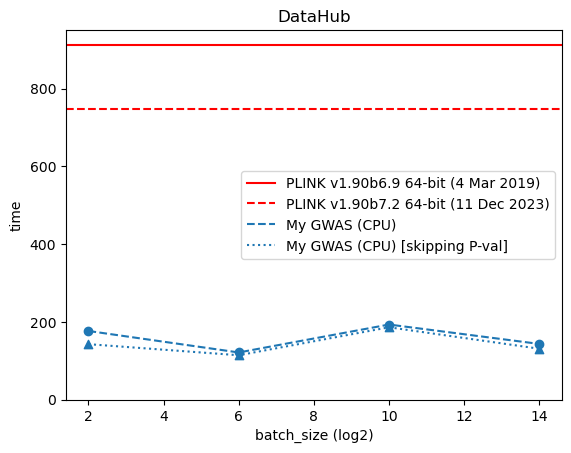
\includegraphics[width=0.3\textwidth]{../datahub.png}
      \caption{\label{fig:frog}This frog was uploaded via the file-tree menu.}
\end{figure}


\section{Discussion}
: outline any challenges you faced or potential future directions you would pursue if you kept working on this project.

Future work: add support to regress out co-variables, such as 
principle components of population, etc.

\section{Code}
\href{https://github.com/weixiao-zhan/CSE284_ParallelGWAS}
{github repo: https://github.com/weixiao-zhan/CSE284\_ParallelGWAS}

\section{References}



\subsection{How to add Citations and a References List}

You can simply upload a \verb|.bib| file containing your BibTeX entries, created with a tool such as JabRef. You can then cite entries from it, like this: \cite{greenwade93}. Just remember to specify a bibliography style, as well as the filename of the \verb|.bib|. You can find a \href{https://www.overleaf.com/help/97-how-to-include-a-bibliography-using-bibtex}{video tutorial here} to learn more about BibTeX.

If you have an , you can also import your Mendeley or Zotero library directly as a \verb|.bib| file, via the upload menu in the file-tree.

\bibliographystyle{alpha}
\bibliography{sample}

\end{document}